\documentclass{article}
\usepackage{amsfonts,enumerate,zed-csp}
%%%%%%%%%%%%%%%%%%%%%%%%%%%%%%%%%%%%%%%%%%%%%%%%%%%%%%%%%%%%%%%%
%  6.826 (POCS Seminar) macro file for handouts and problem sets.
%
% You should save this file as handout.tex
%
% Your main LaTeX file should look like this:
%
%        \documentstyle[12pt]{article}
%
%        %%%%%%%%%%%%%%%%%%%%%%%%%%%%%%%%%%%%%%%%%%%%%%%%%%%%%%%%%%%%%%%%
%  6.826 (POCS Seminar) macro file for handouts and problem sets.
%
% You should save this file as handout.tex
%
% Your main LaTeX file should look like this:
%
%        \documentstyle[12pt]{article}
%
%        %%%%%%%%%%%%%%%%%%%%%%%%%%%%%%%%%%%%%%%%%%%%%%%%%%%%%%%%%%%%%%%%
%  6.826 (POCS Seminar) macro file for handouts and problem sets.
%
% You should save this file as handout.tex
%
% Your main LaTeX file should look like this:
%
%        \documentstyle[12pt]{article}
%
%        \input{handout}
%%%%%%%%%%%%%%%%%%%%%%%%%%%%%%%%%%%%%%%%%%%%%%%%%%%%%%%%%%%%%%%%

\oddsidemargin 0in
\evensidemargin 0in
\marginparwidth 40pt
\marginparsep 10pt
\topmargin 0pt
\headsep 0in
\headheight 0in
\textheight 8.5in
\textwidth 6in
\brokenpenalty=10000

% \handout{number}{date}{title}

\newcommand{\handout}[3]{


\begin{center}
\rule{\textwidth}{.0075in} \\
\rule[3mm]{\textwidth}{.0075in}\\

CMU 17-651\hfill Models of Software Systems\hfill Fall 2018\\[3ex]

{\Large\bf #3}\\[3ex]

Dario A Lencina-Talarico \hfill {\bf Handout #1} \hfill #2

\rule{\textwidth}{.0075in} \\
\rule[3mm]{\textwidth}{.0075in} \\
\end{center}

}

% \homework{number}{date}{title}{due-date}
\newcommand{\homework}[4]{

\begin{center}
\rule{\textwidth}{.0075in} \\
\rule[3mm]{\textwidth}{.0075in}\\

CMU 17-651\hfill Models of Software Systems\hfill Fall 2018\\[3ex]

{\Large\bf #3} \\[3ex]

Dario A Lencina Talarico \hfill  #1  \hfill Due: #2\\

\rule{\textwidth}{.0075in} \\
\rule[3mm]{\textwidth}{.0075in} \\
\end{center}

%\noindent
%{\bf Due date: #4}

}

% \solutionset{number}{date}{title}{due-date}
\newcommand{\solutionset}[4]{

\begin{center}
\rule{\textwidth}{.0075in} \\
\rule[3mm]{\textwidth}{.0075in}\\

CMU 17-651\hfill Models of Software Systems\hfill Fall 2016\\[3ex]

{\Large\bf #3} \\[3ex]

Garlan  \hfill  Solutions for Homework #1  \hfill  #2\\

\rule{\textwidth}{.0075in} \\
\rule[3mm]{\textwidth}{.0075in} \\
\end{center}

%\noindent
%{\bf Due date: #4}

}

% \problem{problem-number}
\newcommand{\problem}[1]{
\vspace{2ex}
\noindent
{\bf Problem #1.}

}

% \solution{solution-number}{points}
\newcommand{\solution}[2]{
\vspace{3ex}
\noindent
{\bf Problem #1}  (#2 points)

}

\newcommand{\cscomment}{
\vspace{1ex}
\noindent Comments: }

% \parts{part-alphabet}{points}
\newcommand{\parts}[2]{
\vspace{2ex}
\noindent
{\bf (#1)}  (#2 points)

}

% \problems{problems-number}{points}
\newcommand{\problems}[2]{
\vspace{3ex}
\noindent
{\bf Problem #1}  (#2 points)

}

\newenvironment{symbolfootnotes}{\def\thefootnote{\fnsymbol{footnote}}}{}

%%%%%%%%%%%%%%%%%%%%%%%%%%%%%%%%%%%%%%%%%%%%%%%%%%%%%%%%%%%%%%%%

\oddsidemargin 0in
\evensidemargin 0in
\marginparwidth 40pt
\marginparsep 10pt
\topmargin 0pt
\headsep 0in
\headheight 0in
\textheight 8.5in
\textwidth 6in
\brokenpenalty=10000

% \handout{number}{date}{title}

\newcommand{\handout}[3]{


\begin{center}
\rule{\textwidth}{.0075in} \\
\rule[3mm]{\textwidth}{.0075in}\\

CMU 17-651\hfill Models of Software Systems\hfill Fall 2018\\[3ex]

{\Large\bf #3}\\[3ex]

Dario A Lencina-Talarico \hfill {\bf Handout #1} \hfill #2

\rule{\textwidth}{.0075in} \\
\rule[3mm]{\textwidth}{.0075in} \\
\end{center}

}

% \homework{number}{date}{title}{due-date}
\newcommand{\homework}[4]{

\begin{center}
\rule{\textwidth}{.0075in} \\
\rule[3mm]{\textwidth}{.0075in}\\

CMU 17-651\hfill Models of Software Systems\hfill Fall 2018\\[3ex]

{\Large\bf #3} \\[3ex]

Dario A Lencina Talarico \hfill  #1  \hfill Due: #2\\

\rule{\textwidth}{.0075in} \\
\rule[3mm]{\textwidth}{.0075in} \\
\end{center}

%\noindent
%{\bf Due date: #4}

}

% \solutionset{number}{date}{title}{due-date}
\newcommand{\solutionset}[4]{

\begin{center}
\rule{\textwidth}{.0075in} \\
\rule[3mm]{\textwidth}{.0075in}\\

CMU 17-651\hfill Models of Software Systems\hfill Fall 2016\\[3ex]

{\Large\bf #3} \\[3ex]

Garlan  \hfill  Solutions for Homework #1  \hfill  #2\\

\rule{\textwidth}{.0075in} \\
\rule[3mm]{\textwidth}{.0075in} \\
\end{center}

%\noindent
%{\bf Due date: #4}

}

% \problem{problem-number}
\newcommand{\problem}[1]{
\vspace{2ex}
\noindent
{\bf Problem #1.}

}

% \solution{solution-number}{points}
\newcommand{\solution}[2]{
\vspace{3ex}
\noindent
{\bf Problem #1}  (#2 points)

}

\newcommand{\cscomment}{
\vspace{1ex}
\noindent Comments: }

% \parts{part-alphabet}{points}
\newcommand{\parts}[2]{
\vspace{2ex}
\noindent
{\bf (#1)}  (#2 points)

}

% \problems{problems-number}{points}
\newcommand{\problems}[2]{
\vspace{3ex}
\noindent
{\bf Problem #1}  (#2 points)

}

\newenvironment{symbolfootnotes}{\def\thefootnote{\fnsymbol{footnote}}}{}

%%%%%%%%%%%%%%%%%%%%%%%%%%%%%%%%%%%%%%%%%%%%%%%%%%%%%%%%%%%%%%%%

\oddsidemargin 0in
\evensidemargin 0in
\marginparwidth 40pt
\marginparsep 10pt
\topmargin 0pt
\headsep 0in
\headheight 0in
\textheight 8.5in
\textwidth 6in
\brokenpenalty=10000

% \handout{number}{date}{title}

\newcommand{\handout}[3]{


\begin{center}
\rule{\textwidth}{.0075in} \\
\rule[3mm]{\textwidth}{.0075in}\\

CMU 17-651\hfill Models of Software Systems\hfill Fall 2018\\[3ex]

{\Large\bf #3}\\[3ex]

Dario A Lencina-Talarico \hfill {\bf Handout #1} \hfill #2

\rule{\textwidth}{.0075in} \\
\rule[3mm]{\textwidth}{.0075in} \\
\end{center}

}

% \homework{number}{date}{title}{due-date}
\newcommand{\homework}[4]{

\begin{center}
\rule{\textwidth}{.0075in} \\
\rule[3mm]{\textwidth}{.0075in}\\

CMU 17-651\hfill Models of Software Systems\hfill Fall 2018\\[3ex]

{\Large\bf #3} \\[3ex]

Dario A Lencina Talarico \hfill  #1  \hfill Due: #2\\

\rule{\textwidth}{.0075in} \\
\rule[3mm]{\textwidth}{.0075in} \\
\end{center}

%\noindent
%{\bf Due date: #4}

}

% \solutionset{number}{date}{title}{due-date}
\newcommand{\solutionset}[4]{

\begin{center}
\rule{\textwidth}{.0075in} \\
\rule[3mm]{\textwidth}{.0075in}\\

CMU 17-651\hfill Models of Software Systems\hfill Fall 2016\\[3ex]

{\Large\bf #3} \\[3ex]

Garlan  \hfill  Solutions for Homework #1  \hfill  #2\\

\rule{\textwidth}{.0075in} \\
\rule[3mm]{\textwidth}{.0075in} \\
\end{center}

%\noindent
%{\bf Due date: #4}

}

% \problem{problem-number}
\newcommand{\problem}[1]{
\vspace{2ex}
\noindent
{\bf Problem #1.}

}

% \solution{solution-number}{points}
\newcommand{\solution}[2]{
\vspace{3ex}
\noindent
{\bf Problem #1}  (#2 points)

}

\newcommand{\cscomment}{
\vspace{1ex}
\noindent Comments: }

% \parts{part-alphabet}{points}
\newcommand{\parts}[2]{
\vspace{2ex}
\noindent
{\bf (#1)}  (#2 points)

}

% \problems{problems-number}{points}
\newcommand{\problems}[2]{
\vspace{3ex}
\noindent
{\bf Problem #1}  (#2 points)

}

\newenvironment{symbolfootnotes}{\def\thefootnote{\fnsymbol{footnote}}}{}

\newcommand{\Until}{\,\mathcal{U}\,}
\newcommand{\Next}{\bigcirc}
\usepackage{graphicx}
\begin{document}

\homework{}{14 November 2016}{Homework \#12: LTL and FSP Concurrency}{}

\begin{enumerate}
\item For each of the following pairs, either argue (informally) why they are equivalent, or provide a counterexample trace that shows they are not equivalent.

    {\sc Note} regarding counterexamples: To show that, for example, $\Box (p \land q)$ and $\Box (p \lor q)$ are {\em not} equivalent we provide the counterexample trace $\langle (p,\neg q), (p,\neg q), \ldots \rangle$. This trace is read as follows: ``in state 1 $p$ is true and $q$ is false, in state 2 $p$ is true and $q$ is false, and so on for the entire trace." $\Box (p \lor q)$ is true for the given trace since $p$ is true in every state of the trace (and hence so is $p \lor q$), but $\Box (p \land q)$ is not true since that would require both $p$ and $q$ to be true in every state of the trace.
\begin{enumerate}
\item \makebox[1.5in][l]{$\Diamond p\land\Diamond q$}   $\Diamond(p\land\Diamond q)\lor\Diamond(q\land\Diamond p)$
\item \makebox[1.5in][l]{$\Diamond p\land\Diamond q$}  $\Diamond(p\land q)$
\item \makebox[1.5in][l]{$\Box(p\lor q)$} $\Box p \lor \Box q$
\item \makebox[1.5in][l]{$(p\land q)\Until r$} $(p\Until r)\land (q\Until r)$
\end{enumerate}
\item Assuming that the following are true of $\sigma$:
\begin{itemize}
\item $\Box((p\implies q)\lor s)$
\item $(\sigma,3)\models\Box p $
\item $(\sigma,3)\models\Next(q\land\Next\Box r) $
\item $(\sigma,4)\models\Box(r\implies\neg q) $
\end{itemize}
which of the following are true, which are false, and which could be either?
\begin{enumerate}
\item $(\sigma,5)\models q$
\item $(\sigma,4)\models s$
\item $(\sigma,5)\models s$
\item $(\sigma,3)\models q\lor s$
\item $(\sigma,4)\models r$
\end{enumerate}


\item The following is an FSP model of the alternating-bit communication protocol
over an unreliable link:

\begin{small}
\begin{verbatim}
const Max = 1 range Msg = 0..Max

SENDER = SENDER[0], SENDER[i:Msg] = (
    send_msg[i] -> (
        msg_received[i] -> (
            // proceed to send the next message
            ack_received[i] -> SENDER[(i + 1) % (Max + 1)]
            |
            // retransmit
            ack_timeout[i] -> SENDER[i]
        )
        |
        // retransmit
        msg_timeout[i] -> SENDER[i]
    )
).

RECEIVER = RECEIVER[0][1], RECEIVER[i:Msg][j:Msg] = (
    msg_received[i] -> send_ack[i] -> ( // process the currently expected message
        ack_received[i] -> RECEIVER[(i + 1) % (Max + 1)][i]
        |
        ack_timeout[i] -> RECEIVER[(i + 1) % (Max + 1)][i]
    )
    |
    msg_received[j] -> send_ack[j] -> ( // process the previously expected message
        ack_received[j] -> RECEIVER[(j + 1) % (Max + 1)][j]
        |
        ack_timeout[j] -> RECEIVER[(j + 1) % (Max + 1)][j]
    )
).

||ALTBITPROTOCOL = (SENDER || RECEIVER).
\end{verbatim}
\end{small}

As shown by the model, this protocol follows the ``stop-and-wait''
style. That is, a new message is not transmitted from the sender to
the receiver unless (1)~the receiver has sent back an acknowledgment
and (2)~the sender has received that acknowledgement. Since, the
link is unreliable, both messages and acknowledgments may be lost at
any time. Also, notice that the link is ``half-duplex''---meaning
that transmissions go over one direction at a time.

\begin{enumerate}
\item Use LTSA to check if this protocol is deadlock free. Briefly explain why the protocol is deadlock free or why it is not. \\
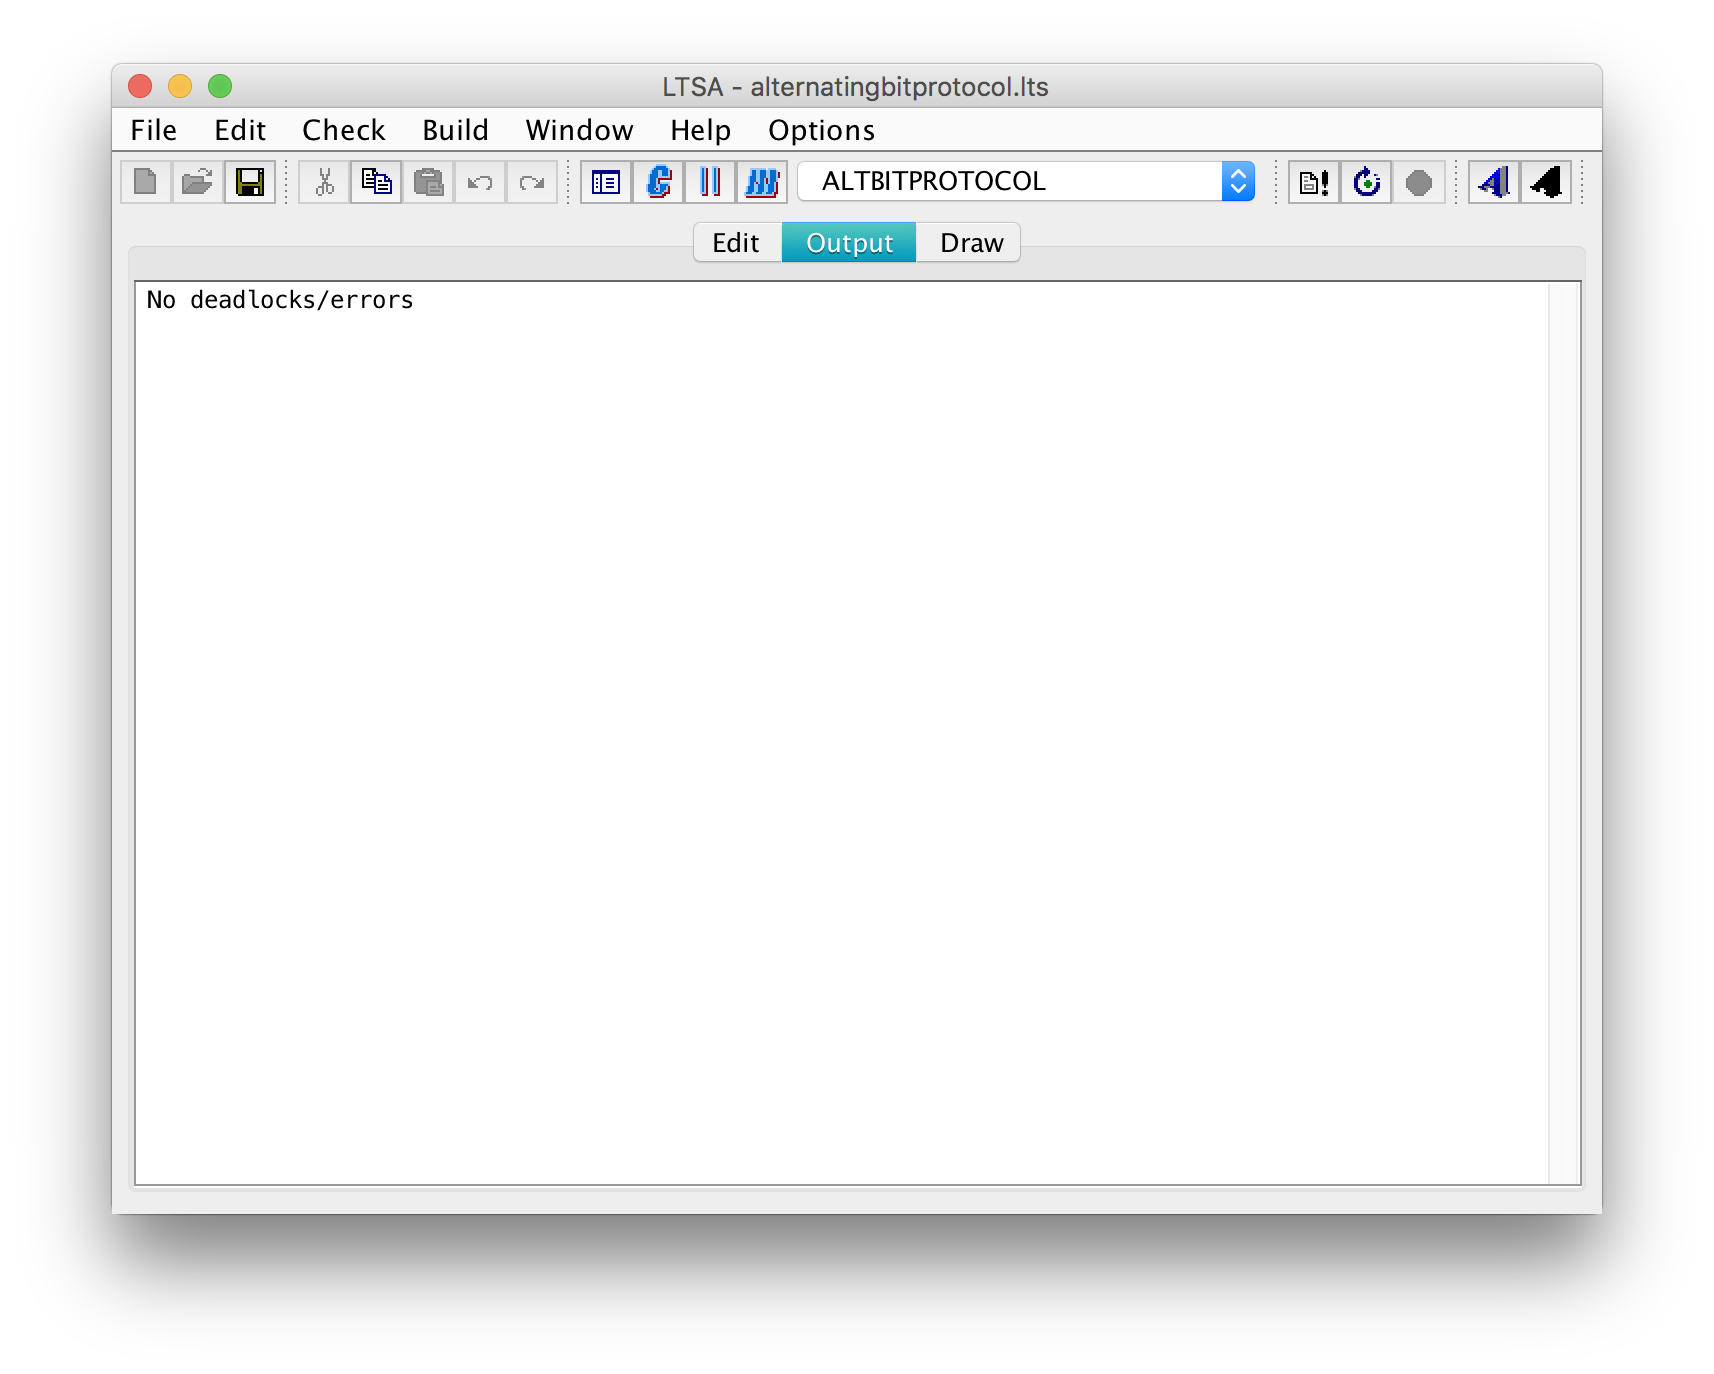
\includegraphics[scale=0.5]{deadlocks.png}

\item Define fluents \verb"MSG_SENT" and \verb"ACK_SENT" and an FLTL
formula which uses those fluents and states that every message
transmitted by the sender is eventually retrieved by the receiver.

\item Use LTSA to check if the protocol satisfies your LTL property. Briefly explain why the property is satisfied or why it is not.

\item Modify the model by removing the \verb"*_timeout" transition
choices and rerun LTSA to check if the modified protocol is deadlock
free. Briefly explain why the modified protocol is deadlock free or why it is not.
\end{enumerate}
NOTE: For every question in which you are asked to use the LTSA LTL
property checker, you need to include the actual resulting output of
the checker.

\end{enumerate}


\end{document}
